\section{Problemformulering}
\label{sec:problemformulering}

Et Pan \& Tilt-system (PTS) skal opbygges til tracking af en lerdue i English Skeet (ES).

PTS dimensioneres til en konkurrence i ES og er afgrænset til et enkelt tilfælde:
Afskydning fra ”High-House” med PTS placeret på station 4, jf. figur \ref{fig:ES}.
\begin{figure}[th!]
\centering
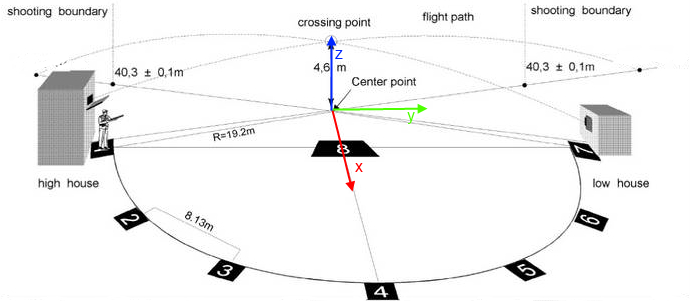
\includegraphics[width=1\textwidth]{./graphics/skeet_diagram_cropped_axes}
\caption[tekst i indholdsfortegnelsen]{figurtekst}
\label{fig:ES}
\end{figure}	
PTS' udgangsposition er at pan-rammen står vinkelret på x-aksen jf. figur \ref{fig:ES},
og at tilt-rammen er lodret (parallel med yz-planet).

Trackingen skal forestille at have til formål at assistere i nedskydningen af lerduen,
og man skal således forestille sig et gevær monteret på tilt-rammen:
Et tænkt masseløst gevær placeret i skæringspunktet mellem pan- og tilt-akserne står vinkelret
på tilt-planet, og skal skyde lerduen jf. reglerne for ES, dvs. inden den når "low house" jf. figur \ref{fig:ES}.
Da man har to skud til rådighed, er det et krav at trackingen foretaget af PTS har stabiliseret sig på lerduen
i tide, så man kan nå at affyre to skud.

Det tænkte gevær er et 12 gauge haglgevær med Skeet Choke.

Lerduens koordinater i det kartesiske koordinatsystem som vist på figur \ref{fig:ES}
vil med en frekvens på 60 [Hz] blive givet som input til systemet.

Som angivet i projektoplægget skal reguleringen foregå på en microcontroller,
mens motorpositionsbestemmelse skal foregå på en FPGA.